%%%%%%%%%%%%%%%%%%%%%%%%%%%%%%%%%%%%%%%%%
% University/School Laboratory Report
% LaTeX Template
% Version 3.0 (4/2/13)
%
% This template has been downloaded from:
% http://www.LaTeXTemplates.com
%
% Original author:
% Linux and Unix Users Group at Virginia Tech Wiki 
% (https://vtluug.org/wiki/Example_LaTeX_chem_lab_report)
%
% License:
% CC BY-NC-SA 3.0 (http://creativecommons.org/licenses/by-nc-sa/3.0/)
%
%%%%%%%%%%%%%%%%%%%%%%%%%%%%%%%%%%%%%%%%%

%----------------------------------------------------------------------------------------
%	PACKAGES AND DOCUMENT CONFIGURATIONS
%----------------------------------------------------------------------------------------

\documentclass{article}

\usepackage[version=3]{mhchem} % Package for chemical equation typesetting
\usepackage{siunitx} % Provides the \SI{}{} command for typesetting SI units
\usepackage{fullpage}
\usepackage{subcaption}
\setlength{\parskip}{3mm}
\usepackage[titletoc,title]{appendix}
\usepackage{xfrac}
\usepackage{tikz}
\usepackage{tablefootnote}
\usepackage{epstopdf}
\usepackage{enumitem}
\usepackage{etoolbox}
\usepackage{wrapfig}
\usepackage{longtable}
\usepackage{array}
\usepackage{setspace}
\usepackage{multirow}
\usepackage[bookmarks]{hyperref}
\usepackage{listings}
\patchcmd{\thebibliography}{\section*{\refname}}{}{}{}

\usepackage{graphicx} % Required for the inclusion of images


\usepackage{sourcecodepro}
\usepackage[default]{sourcesanspro}
\usepackage[T1]{fontenc}

% code command for including code snippets inline
% (fake verbatim, so all special character should be escaped,
% or textmode equivalents of special characters should be used)
\newcommand{\code}[1]{
    \begin{tikzpicture}[baseline=0ex] 
        \node[anchor=base, text height=1em, text depth=1ex, inner ysep=0pt, draw=black!13, fill=black!3, rounded corners=2pt] at (0,0) {
            \footnotesize\texttt{#1}
        }; 
    \end{tikzpicture}
}

% button command for including code snippets inline
% (fake verbatim, so all special character should be escaped,
% or textmode equivalents of special characters should be used)
\newcommand{\button}[1]{
    \begin{tikzpicture}[baseline=0ex] 
        \node[anchor=base, text height=1em, text depth=1ex, inner ysep=0pt, draw=black!13, fill=black!3, rounded corners=2pt] at (0,0) {
            \footnotesize{#1}
        }; 
    \end{tikzpicture}
}

\lstset{
  showspaces=false,
  showtabs=false,
  breaklines=true,
  showstringspaces=false,
  breakatwhitespace=true,
  stringstyle=\color{greenstrings},
  basicstyle=\ttfamily\color{grey}
}

%\setlength\parindent{0pt} % Removes all indentation from 

\renewcommand{\arraystretch}{1.5} % Fix the table sizes
\addtocontents{toc}{\protect\setstretch{-1}}


%\usepackage{times} % Uncomment to use the Times New Roman font

%----------------------------------------------------------------------------------------
%	DOCUMENT INFORMATION
%----------------------------------------------------------------------------------------

\title{\includegraphics[width=.3\textwidth]{/Users/ben/Dropbox/Resources/UVicLogo/UVicLogo} \\ \vspace{7mm} Milestone 3 \\ SENG 310} % Title


\author{UVic Enhancement Suite} % Author name

\date{\today} % Date for the report

\raggedright
\begin{document}

\maketitle % Insert the title, author and date

\begin{center}
\begin{tabular}{l r}
Team Members & Ben Hawker \\
 & Brendon Earl \\
 & Clair Xu \\
 & David Draker \\
 & Kent MacDonald \\
Instructor: & Erini Kalliamvakou  % Instructor/supervisor
\end{tabular}
\end{center}

% If you wish to include an abstract, uncomment the lines below
% \begin{abstract}
% Abstract text
% \end{abstract}

\tableofcontents
\pagebreak

%--------------------------------------------------------------------------------
%	SCENARIOS
%--------------------------------------------------------------------------------

\section{User Stories - Conventional Services}

This is a quick recap of the two user stories of our two personas. These stories are intended to be representative of common tasks for UVic students. The stories  use the context of the current UVic web services to provide guidance for potential issues.

\subsection{Scholarship Application}

Amy, like many other university students is starting to run out of money by her 3rd year of university. She decides to apply for a few scholarships. After spending a few hours on one of the applications, the form says to attach a copy of her "Official Transcript" and "Summary of Tuition Fees". Amy spends the rest of her night attempting to find these documents on the UVIC myPage website. Unfortunately, due to the confusing layout of the website she is unsuccessful, and unable to submit the application.

\subsection{First Class}

It's Tuesday, Daniel has just started his first semester of classes at UVic. He needs to get to his first class, MATH 100. He finds the course on his timetable but doesn't know what DTB is. He finds out it's the David Turpin Building from the website but then someone says to "just go to SSM" and he gets confused. Not sure where his class is Daniel ends up in the David Strong Building and sits through a full hour and twenty minutes of ECON 103c.

%--------------------------------------------------------------------------------
%	Use Cases
%--------------------------------------------------------------------------------

\section{Use Cases}

Broadly, there are two use cases for the UVic web services,

\begin{description}
  \item[Retrieving Information] Frequently UVic students require information about their, finances, grades or schedule from their web services. This use case is exemplified by both user stories.
  \item[Submitting Information] UVic students also need submit information either to notify to University of something or to update personal information. This use case is shown in Amy's user story.
\end{description}

There are many tasks that fall into these use cases not all of which are included. However, most in practice are very similar to one of the use cases listed below.

\section{User Flows}

This section contains the flows for Amy and Daniel as they complete their tasks using the improved UVic web services.

\subsection{Scholarship Application}

\textbf{Background:} Amy, like many other university students is starting to run out of money by her 3rd year of university. She decides to apply for a few scholarships. After spending a few hours on one of the applications, the form says to attach a copy of her "Official Transcript" and "Summary of Tuition Fees".

\renewcommand*{\arraystretch}{12}
\begin{longtable}[t]{p{10cm}>{\raggedright\arraybackslash}p{4cm}}
     $\vcenter{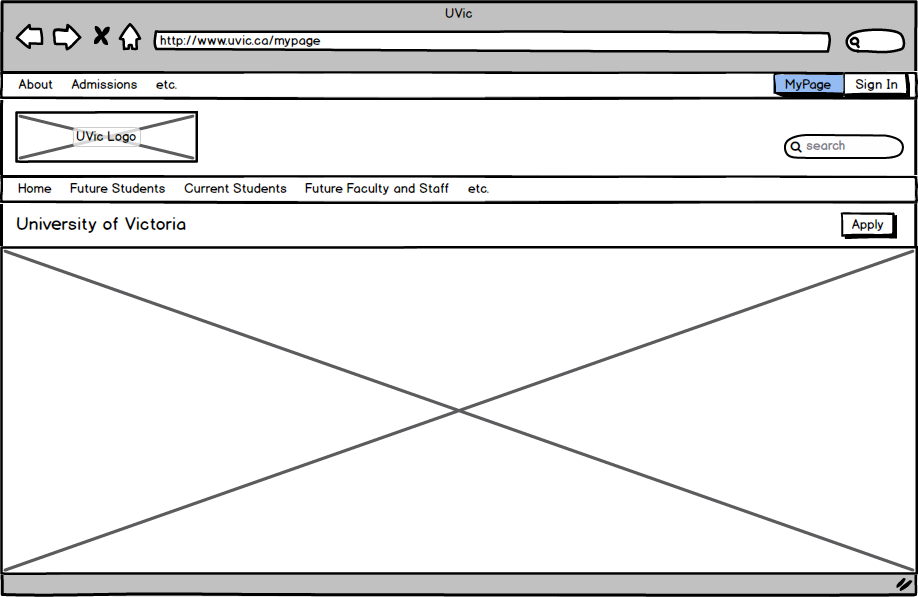
\includegraphics[width=\linewidth]{img/UVic-Start}}$ & Amy starts by opening the UVic Website (uvic.ca) and clicks \button{myPage}. \\
     $\vcenter{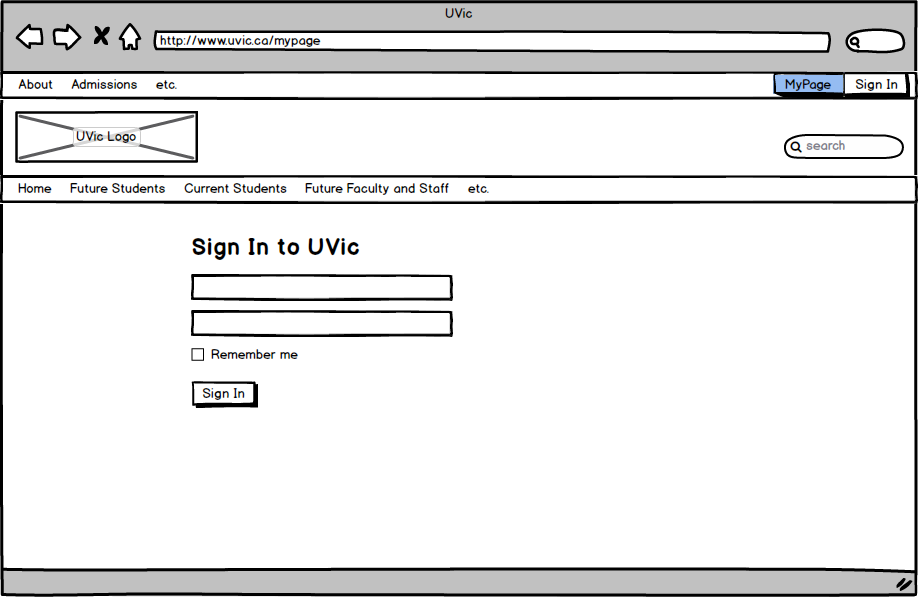
\includegraphics[width=\linewidth]{img/UVic-Sign-In}}$ & Amy signs in using her Netlink ID and password. \\
     $\vcenter{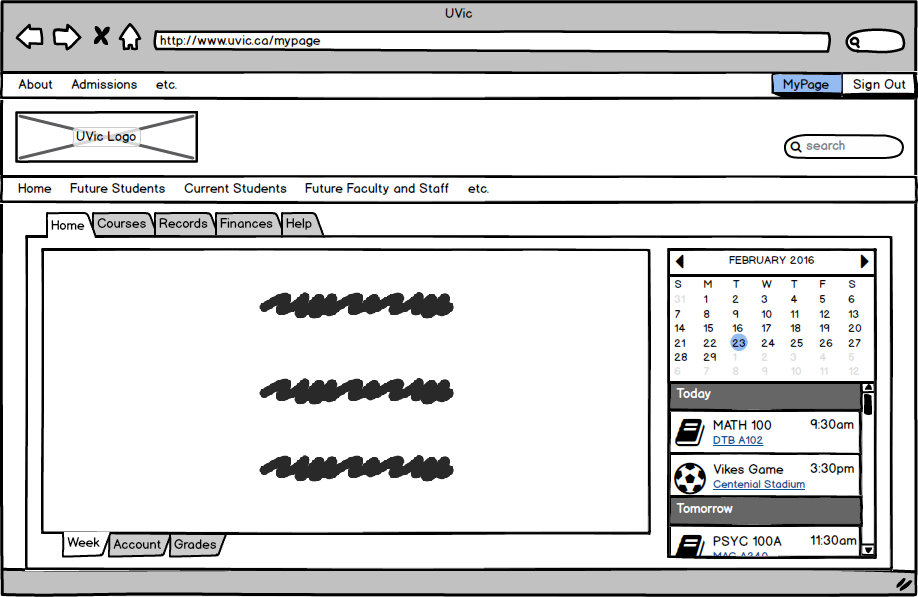
\includegraphics[width=\linewidth]{img/Home}}$ & Amy is redirected to her myPage which provides contextual information about her courses. Amy selects \button{Records}.\\
     $\vcenter{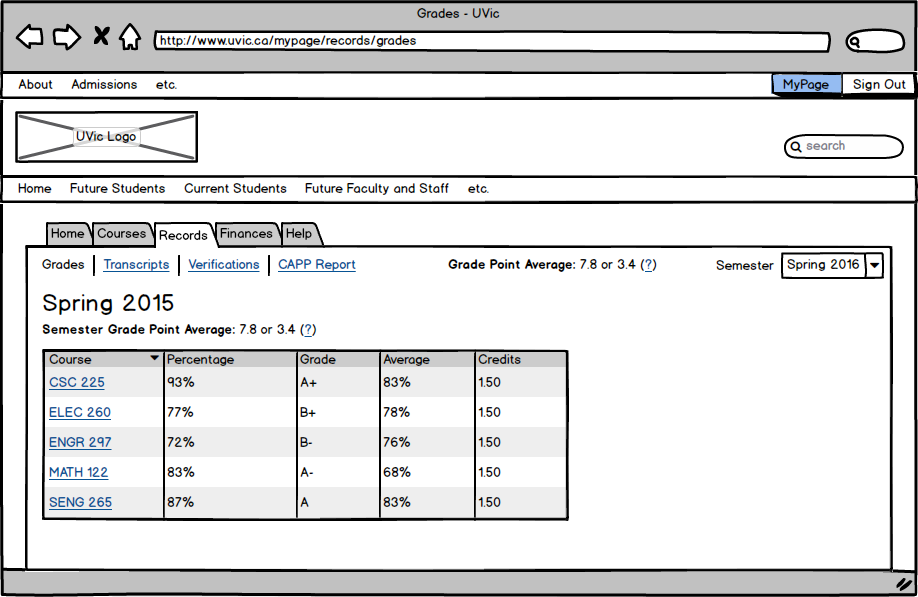
\includegraphics[width=\linewidth]{img/Records-Grades}}$ & Seeing the transcripts button, Amy selects \button{Transcripts}. \\
     $\vcenter{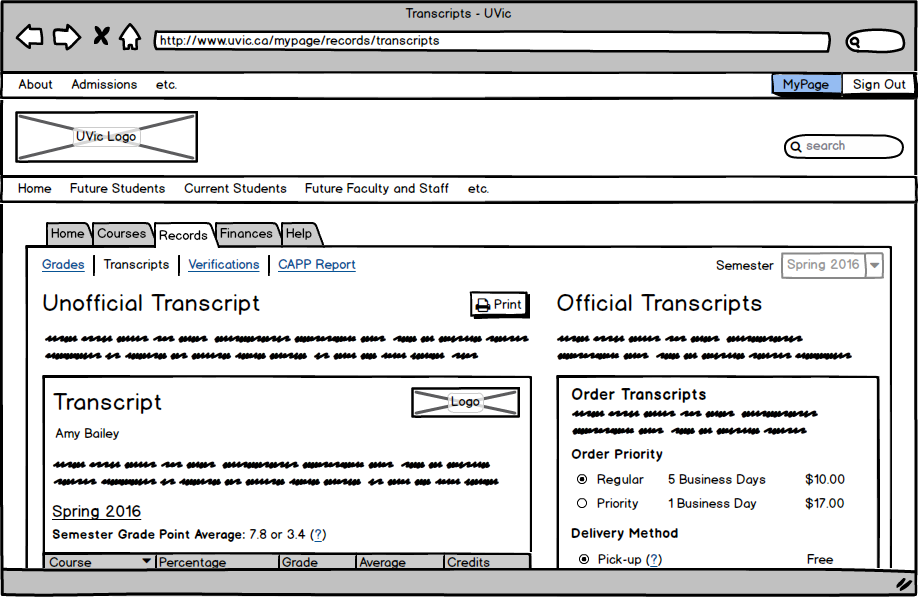
\includegraphics[width=\linewidth]{img/Records-Transcripts}}$ & Amy sees both her Unofficial Transcript and the order form for official transcripts. \\
     $\vcenter{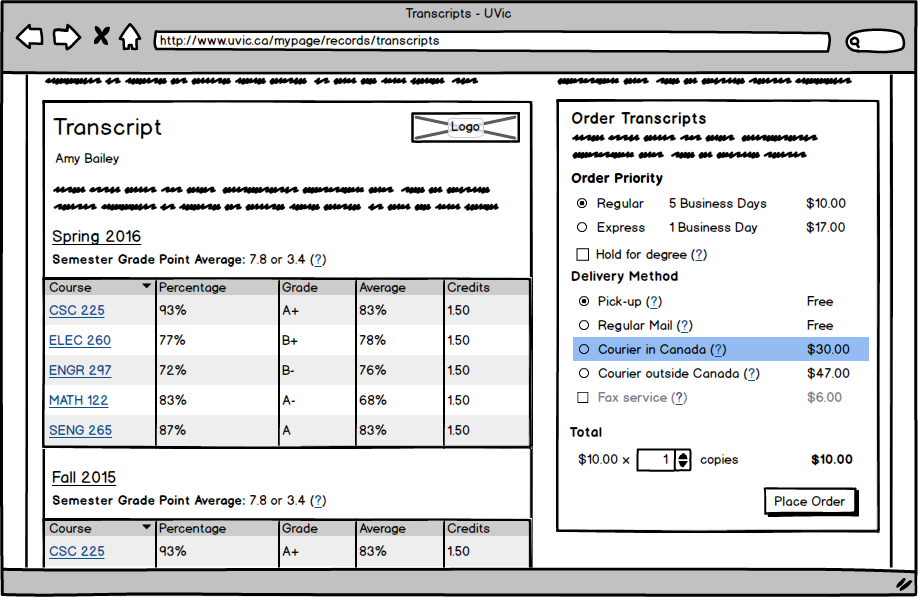
\includegraphics[width=\linewidth]{img/Records-Transcripts-Order}}$ & Amy needs her transcripts delivered as soon as possible, so she chooses couriered and express. \\
     $\vcenter{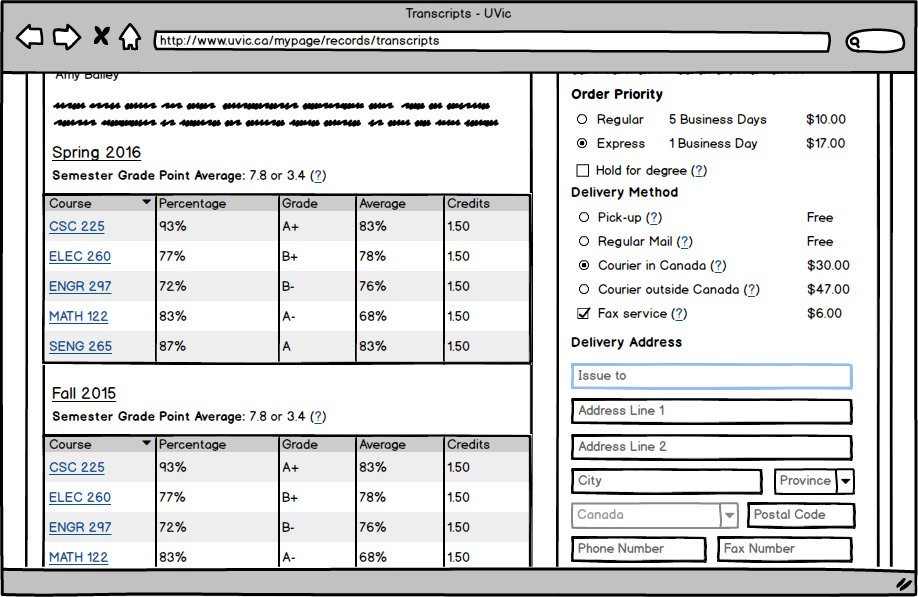
\includegraphics[width=\linewidth]{img/Records-Transcripts-Order-Courier}}$ & Amy adds the delivery address for the scholarship commitee. \\
     $\vcenter{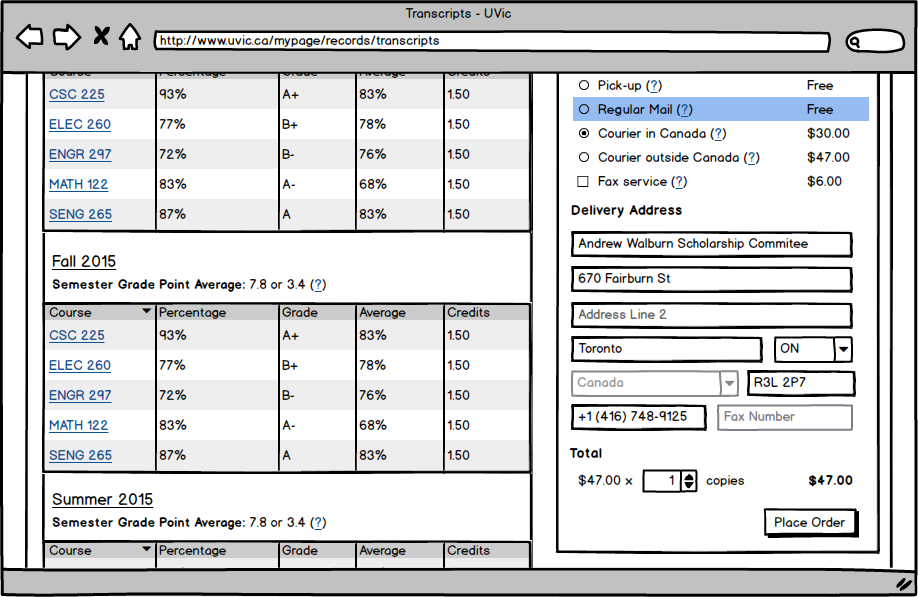
\includegraphics[width=\linewidth]{img/Records-Transcripts-Order-Filled}}$ & Amy sees that the delivery will cost \$47.00 (way too much) and switches to Regular Mail with Fax service. \\
     $\vcenter{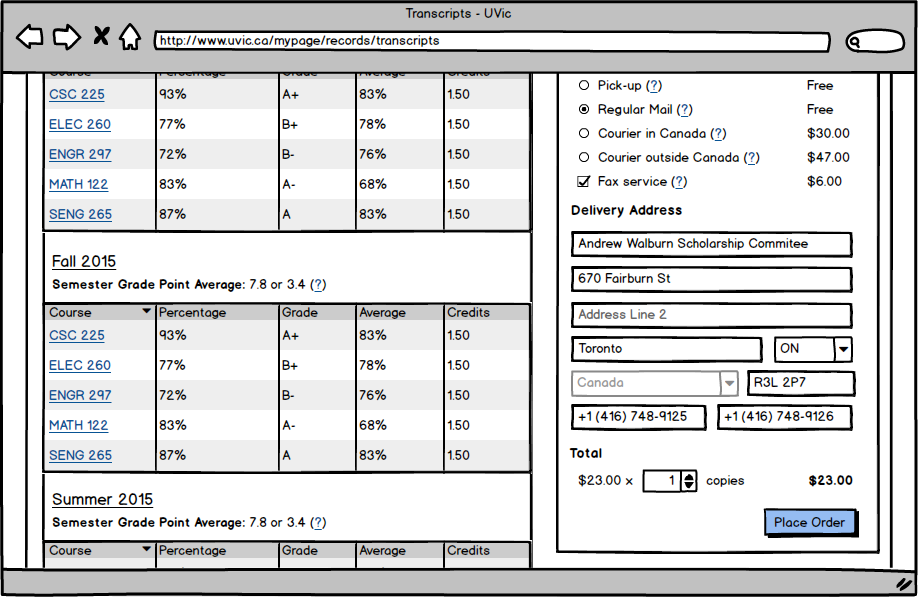
\includegraphics[width=\linewidth]{img/Records-Transcripts-Order-Regular}}$ & Amy's satisfied with her choices and clicks \button{Place Order}. \\
     $\vcenter{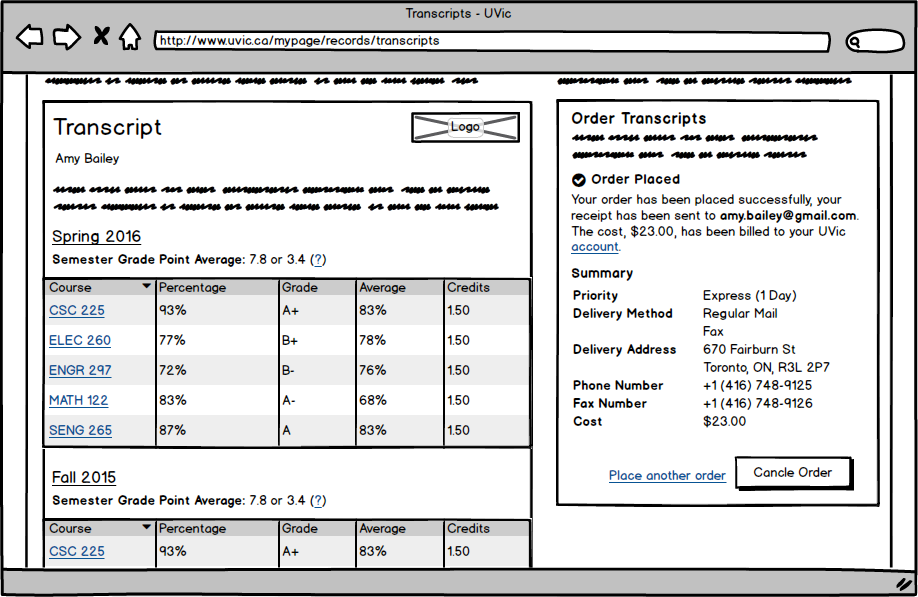
\includegraphics[width=\linewidth]{img/Records-Transcripts-Order-Placed}}$ & Amy reads the summary then moves on to her tuition fees by clicking on the \button{Finances} tab. \\
     $\vcenter{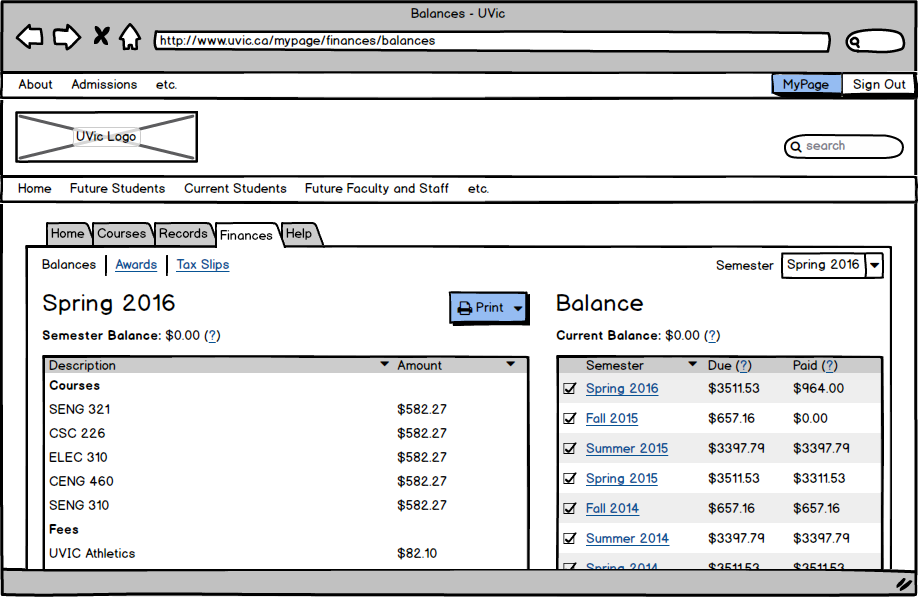
\includegraphics[width=\linewidth]{img/Finances-Balances}}$ & Amy clicks \button{Print}. \\
     $\vcenter{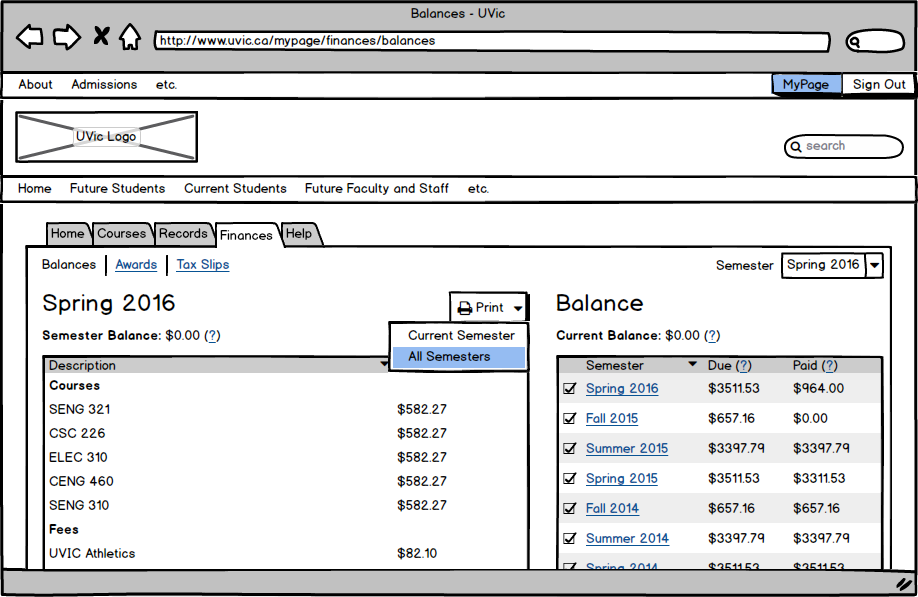
\includegraphics[width=\linewidth]{img/Finances-Balances-Print}}$ & Amy chooses \button{All Semesters}. \\
     $\vcenter{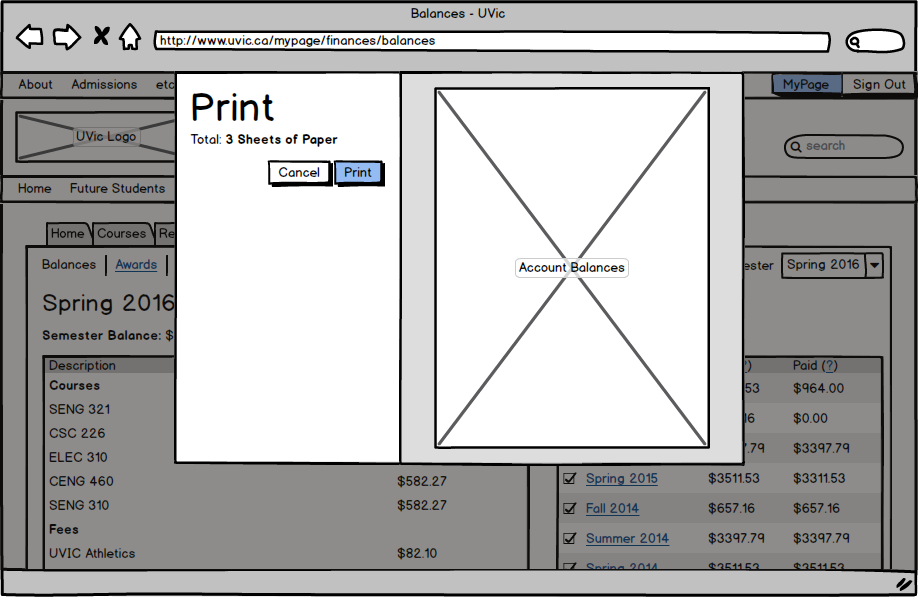
\includegraphics[width=\linewidth]{img/Finances-Balances-Print-Modal}}$ & Amy prints her account summary to PDF using Chrome. \\
\end{longtable}

Amy emails the PDF of her account summary to the Scholarship board. She receives an email later that day (in addition to her receipt) that her transcripts have been faxed to the scholarship board.

\pagebreak
\subsection{First Class}

\textbf{Background:} It's Tuesday, Daniel has just started his first semester of classes at UVic. He needs to get to his first class, MATH 100.

\renewcommand*{\arraystretch}{12}
\begin{longtable}[t]{p{10cm}>{\raggedright\arraybackslash}p{4cm}}
     $\vcenter{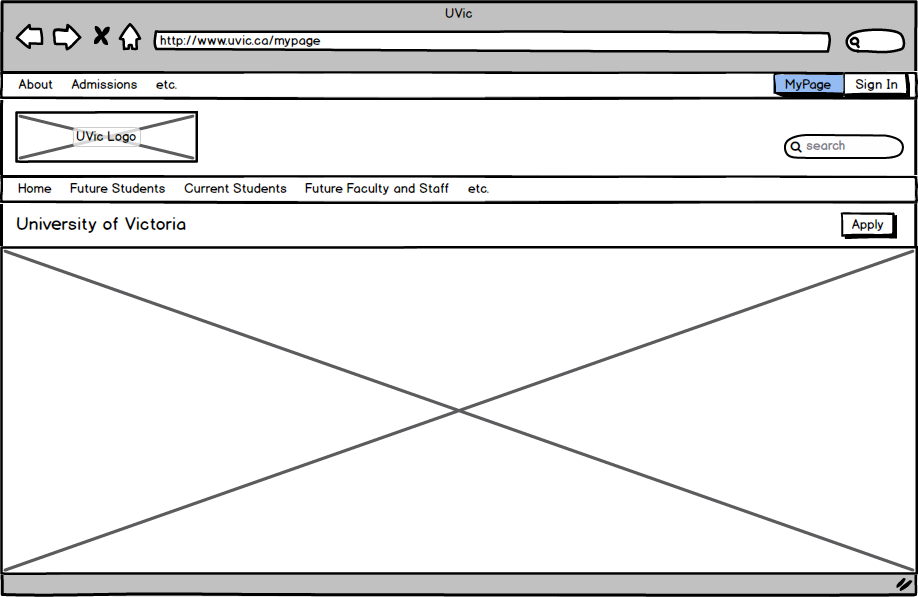
\includegraphics[width=\linewidth]{img/UVic-Start}}$ & Daniel starts by opening the UVic Website (uvic.ca) and clicks \button{myPage}. \\
     $\vcenter{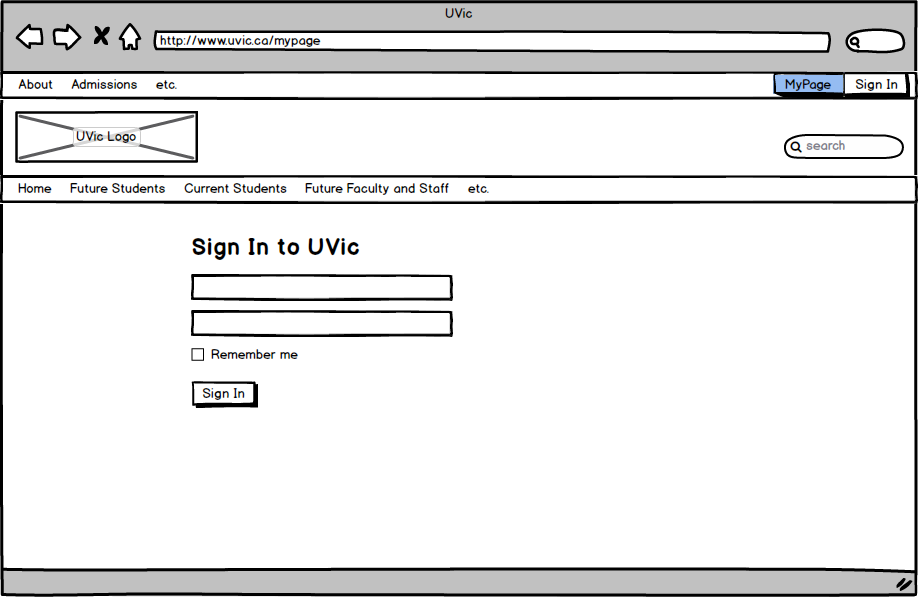
\includegraphics[width=\linewidth]{img/UVic-Sign-In}}$ & Daniel signs in using her Netlink ID and password. \\
     $\vcenter{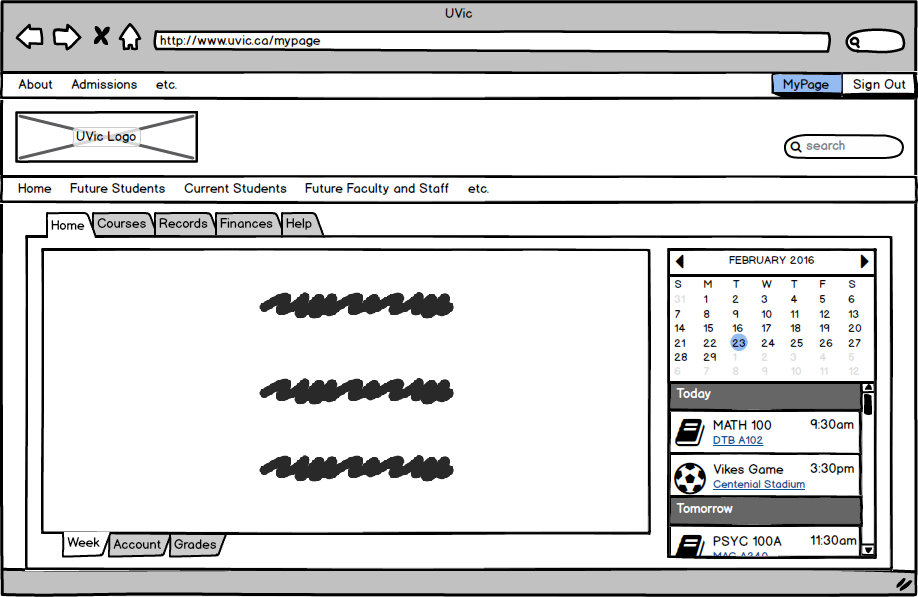
\includegraphics[width=\linewidth]{img/Home}}$ & Daniel is redirected to her myPage which provides contextual information about her courses. He clicks on \button{Math 100}.\\
     $\vcenter{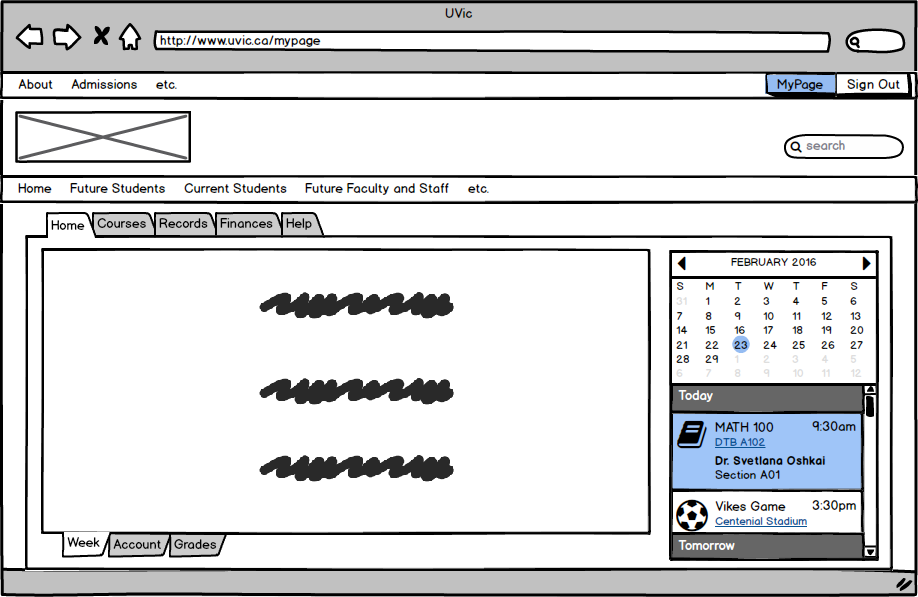
\includegraphics[width=\linewidth]{img/Home-Expanded-Event}}$ & Daniel sees his expanded course information and clicks on the building, \underline{DTB A102}.\\
     $\vcenter{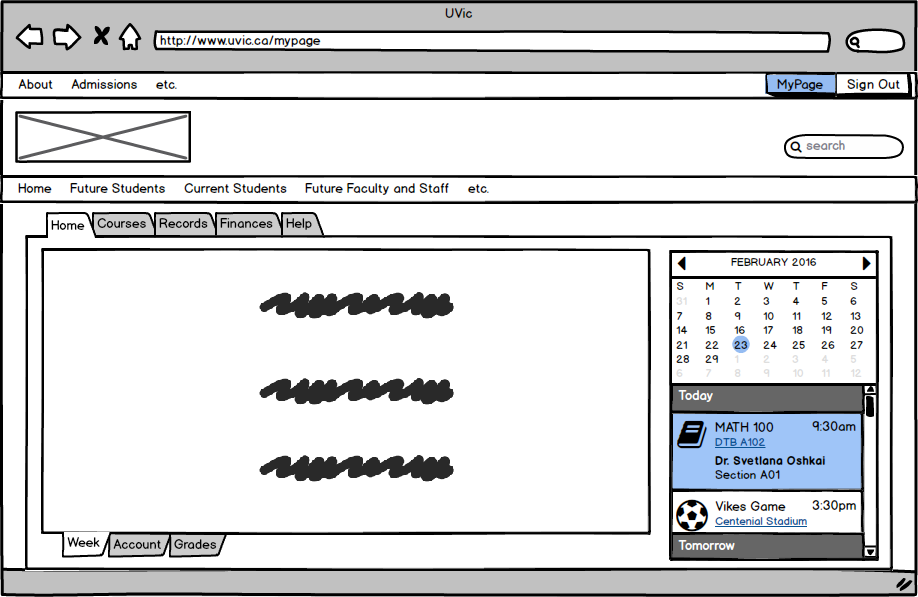
\includegraphics[width=\linewidth]{img/Home-Expanded-Event}}$ & A map to DTB A102 opens in a new tab.\\
\end{longtable}

Daniel notes the location, opening it in maps on his phone, and heads for class. He finds it without difficulty.

%--------------------------------------------------------------------------------
%	Appendices
%--------------------------------------------------------------------------------
%\pagebreak
%\begin{appendices}
%
%\section{User Testing Plan}\label{ap:utesting}
%
%
%\end{appendices}


%--------------------------------------------------------------------------------
%	BIBLIOGRAPHY
%--------------------------------------------------------------------------------

%\section{References}
%
%\bibliographystyle{unsrt}
%



%--------------------------------------------------------------------------------

\end{document}